\documentclass{article}

\usepackage[utf8]{inputenc}
\usepackage[T1]{fontenc}
\usepackage{lipsum}
\usepackage{graphicx}
\usepackage{amsmath}
\usepackage[margin=1in]{geometry}
\usepackage{titlesec}
\usepackage{parskip}
\usepackage{tcolorbox}

\titleformat{\section}
{\LARGE\bfseries}{\thesection}{1em}{}

\titleformat{\subsection}
{\Large\bfseries}{\thesection}{1em}{}

\begin{document}

\pagestyle{empty}

\section*{Erlang}
\large

\subsection*{Tipi di dato}
Come in tutti i linguaggi di programmazione, i dati si dividono in \textbf{predefiniti} o \textbf{definiti dall'utente}, ed \textbf{atomici} o \textbf{non atomici}.

In generale, ogni linguaggio di programmazione mette a disposizione alcuni tipi di dato predefiniti e, a seconda del linguaggio, offre la possibilità di definirne di nuovi.

I nuovi tipi possono essere semplici alias per tipi esistenti, oppure strutture che estendono tipi già presenti (non più semplici alias in questo caso).

Esistono anche tipi di dato più complessi, come i tipi algebrici, che descrivono le possibili forme che un dato può assumere.

Essendo Erlang un linguaggio dinamicamente tipato, non esistono dichiarazioni esplicite di nuovi tipi di dato. Non è presente un costrutto sintattico dedicato alla definizione di tipi. L'utente crea nuove tipologie di dato semplicemente utilizzando i valori in modo coerente.

Un esempio sono i valori booleani, che in Erlang sono rappresentati dagli atomi \texttt{true} e \texttt{false}.

Per quanto riguarda la distinzione tra dati atomici e non atomici, i tipi atomici sono quelli che non contengono altri dati al loro interno.

Un esempio di dato atomico è un numero, mentre un esempio di dato non atomico è una lista, che contiene al suo interno altri elementi.

Tra i dati \textbf{atomici}, in Erlang troviamo:
\begin{itemize}
    \item \textbf{Numeri interi}, sui quali è possibile eseguire le comuni operazioni matematiche.\\
    È importante notare che gli operatori di confronto hanno alcune particolarità sintattiche: mentre l'operatore maggiore o uguale mantiene la forma standard (\texttt{>=}), l'operatore minore o uguale diventa \texttt{=<} per distinguerlo dalla forma di una freccia (essendo Erlang simile al Prolog, le frecce hanno un significato particolare).\\
    Altri operatori di confronto importanti sono l'uguaglianza stretta (\texttt{=:=}) e la disuguaglianza stretta (\texttt{=/=}).
    \item \textbf{Numeri in virgola mobile} (floating point), che quando combinati con numeri interi provocano la conversione implicita del risultato in floating point. È importante notare che il confronto tra un numero intero e uno floating point con \texttt{=:=} restituisce \texttt{false} (ad esempio, \texttt{5.0 =:= 5} è \texttt{false}), poiché rappresentano sequenze di bit differenti. Per un test di uguaglianza meno rigoroso, che considera equivalenti valori numericamente uguali indipendentemente dal tipo, si possono usare gli operatori \texttt{==} o \texttt{/=}.
    \item \textbf{PID} (Process IDentifier), ottenibili chiamando la funzione \texttt{self()}, che identificano univocamente i processi.
    \item \textbf{Reference}, ottenibili chiamando la funzione \texttt{make\_ref()}. Una reference è un valore probabilisticamente unico, progettato per essere diverso da tutte le reference generate in precedenza. Non dovrebbe esistere un algoritmo in grado di prevedere la prossima reference che verrà generata.
    \item \textbf{Porte}. Nel modello ad attori di Erlang, quando è necessario interagire con entità esterne che non sono attori, è possibile avvolgerle in una specie di attore intermediario che permette di comunicare con esse utilizzando i meccanismi di invio e ricezione di messaggi tipici del linguaggio.\\
    Questi attori speciali, che fanno da wrapper a entità esterne, non possiedono tutte le caratteristiche degli attori normali. Ad esempio, non seguono il principio "Let it fail" di Erlang, che normalmente termina tutti gli attori associati a un attore che fallisce.\\
    Quando viene creato questo tipo di attore speciale, gli viene assegnata una porta anziché un PID.
    \item \textbf{Atomi}, che si scrivono normalmente con lettere minuscole. L'idea è che un programma utilizzi un numero limitato di atomi, che verranno rappresentati in memoria come sequenze di bit efficienti.\\
    È possibile racchiudere un atomo contenente spazi tra apici singoli (ad esempio, \texttt{'hello world'}). Da notare che \texttt{'ciao' =:= ciao} restituisce \texttt{true}, poiché sono considerati lo stesso atomo.
    \item \textbf{Caratteri}, anche se in realtà Erlang non ha un tipo carattere. Per invece rappresentare le stringhe viene utilizzata una lista di caratteri. Erlang controlla ogni lista se al suo interno ha valori che rientrano nei valori ASCII dei caratteri.
\end{itemize}

Passando ai dati \textbf{non atomici}, Erlang offre:
\begin{itemize}
    \item \textbf{Tuple}. Si definiscono tra parentesi graffe, con elementi separati da virgole. Un esempio di tupla è \texttt{\{4, \{ciao, 2.0\}, true\}}. Esiste anche la tupla vuota \texttt{\{\}}, utilizzabile quando non si desidera restituire alcun valore significativo.
    \item \textbf{Liste}. Una lista può essere vuota (\texttt{[]}), oppure ha una \textit{testa} (primo elemento) e una \textit{coda} (una lista contenente tutti gli altri elementi).\\
    La testa può essere un valore qualsiasi, mentre la coda è a sua volta una lista.\\
    Un esempio di lista può essere scritto come \texttt{[ 2 | [ 3 | [ 4 | [ ] ] ] ]}, che rappresenta la struttura fondamentale. Per comodità è possibile utilizzare la sintassi semplificata \texttt{[2, 3, 4]}, ma concettualmente la lista è sempre composta da una testa e una coda.
    
    Essendo Erlang un linguaggio dinamicamente tipato, non ci sono garanzie che la coda sia effettivamente una lista. Quando la coda non è una lista, si parla di \textit{lista impropria}, sulla quale non è possibile applicare le normali operazioni previste per le liste.
    
    Le operazioni predefinite sulle liste includono il calcolo della lunghezza, la concatenazione (\texttt{[2, 3] ++ [4, 5]} restituisce \texttt{[2, 3, 4, 5]}) e la sottrazione (\texttt{[2, 3, 4, 5] -- [4, 2]} restituisce \texttt{[3, 5]}). La sottrazione segue una logica insiemistica, quindi in casi come \texttt{[2, 3, 4, 5] -- [4, 2] -- [4]}, il risultato sarà \texttt{[3, 4, 5]} e non \texttt{[3, 5]}.

    Un'altra potente caratteristica delle liste è la \textbf{list comprehension}. Un esempio: \\
    \texttt{[ \{X, Y + 1\} || X <- [1, 2, 3], \{Y, \_\} <- [\{4, 5\}, \{6, 7\}] ].}\\
    Questa espressione restituisce:\\
    \texttt{[ \{1, 5\}, \{1, 7\}, \{2, 5\}, \{2, 7\}, \{3, 5\}, \{3, 7\} ].}
    
    Concettualmente, è come se ci fossero dei cicli for annidati che estraggono valori per X e Y. È anche possibile aggiungere filtri, ad esempio:\\
    \texttt{[ \{X, Y + 1\} || X <- [1, 2, 3], \{Y, \_\} <- [\{4, 5\}, \{6, 7\}], X + Y < 6 ].}\\
    Questa espressione restituisce solamente \texttt{[ \{1, 5\} ]}, poiché solo la coppia \{1, 4\} soddisfa la condizione X + Y < 6.
    \item \textbf{Bit strings}. Erlang offre la possibilità di accedere alla rappresentazione binaria di qualsiasi dato, permettendo di manipolare e analizzare sequenze di bit tramite pattern matching.\\
    Un esempio: \texttt{N = 16\#7A5.} definisce un numero in base 16.\\
    Per accedere alla sua rappresentazione in bit, possiamo usare la sintassi:\\
    \texttt{<< R:4, G:4, B:4 >> = << N:12 >>.}\\
    A questo punto, accedendo a R, G o B otterremo le rispettive sequenze di bit (nell'ordine: 7, 10 e 5).

    Questa funzionalità è particolarmente utile quando si lavora con pacchetti di rete, file binari o per interagire con dispositivi a basso livello, consentendo un controllo preciso sulle sequenze di bit.
\end{itemize}

Rimangono infine le \textbf{funzioni}, note anche come \textbf{chiusure}. Una caratteristica fondamentale dei linguaggi funzionali è che le funzioni sono oggetti di prima classe, manipolabili come qualsiasi altro valore. Una funzione può essere passata come argomento, restituita come risultato, inserita in strutture dati e così via.

In Erlang esistono diverse sintassi per definire funzioni. La prima forma ha la struttura:\\
\texttt{nome\_funzione(lista\_argomenti) -> corpo ... end.} Questa sintassi può essere utilizzata nei file da compilare, ma non direttamente nella shell interattiva.

Una sintassi utilizzabile ovunque impiega la parola chiave \textbf{fun}, ad esempio:\\
\texttt{fun (lista\_argomenti) -> ... end.} Questa è la sintassi per creare una funzione anonima.

È possibile definire funzioni annidate all'interno di altre funzioni. Le funzioni interne hanno accesso alle variabili definite nello scope più esterno (chiusura lessicale).

Un esempio: \texttt{G = fun (X) -> fun (Y) -> X + Y end end.}

Eseguendo \texttt{H = G(2).} e poi \texttt{H(3).}, otterremo il valore \texttt{5}. La variabile X, con valore 2, è stata "catturata" nella chiusura restituita da G.

Per dichiarare una funzione ricorsiva, si può usare la sintassi: \texttt{fun G(N) -> N * G(N) end.}\\
Il nome G è visibile solo all'interno della funzione stessa e non può essere richiamato dall'esterno.

In generale, le funzioni in Erlang utilizzano il pattern matching per selezionare diverse implementazioni in base all'input ricevuto, come accade anche con il costrutto \textit{receive} per la gestione dei messaggi.

Tutti i linguaggi funzionali moderni permettono di definire funzioni per \textbf{casi}, consentendo di scrivere algoritmi in modo conciso e comprensibile, riducendo significativamente la quantità di codice.

Un esempio di funzione definita per casi può essere:\\
\texttt{fun (\{N, 2\}) -> N; (\{ciao, N, M\}) -> N + M; ([\_, \_, \{X, Y\}]) -> X + Y end.}\\
Qui il simbolo \texttt{\_} indica un pattern che corrisponde a qualsiasi valore, il quale viene ignorato (non gli viene assegnato un nome).

Questa è una funzione definita tramite \textit{pattern matching}. In base all'input fornito, verrà eseguito il ramo corrispondente al pattern che corrisponde. Se viene fornito un input che non corrisponde a nessuno dei pattern definiti, verrà sollevata un'eccezione.

È inoltre possibile utilizzare delle \textbf{guardie} per aggiungere condizioni aggiuntive. Dopo il pattern, attraverso la parola chiave \texttt{when}, si possono specificare condizioni che devono essere soddisfatte. Ad esempio:\\
\texttt{fun (\{N, 2\}) when N > 2 -> N; (\{ciao, N, M\}) -> N + M; ([\_, \_, \{X, Y\}]) -> X + Y end.}

Quando più pattern possono corrispondere all'input, l'ordine di valutazione è \textbf{sequenziale} dall'alto verso il basso.

Un aspetto importante delle guardie in Erlang è che il linguaggio si assicura che la loro valutazione non produca effetti collaterali, come l'invio di messaggi o la creazione di nuovi processi. Molti linguaggi moderni non effettuano questo controllo.

In Erlang, le guardie possono contenere solo combinazioni di funzioni predefinite chiamate \textbf{BIF} (Built-In Functions).\\
Questa restrizione rende il linguaggio delle guardie meno espressivo, il che può diventare problematico in casi complessi, come quando si desidera impedire l'attivazione di uno specifico caso in base a condizioni elaborate.

\subsection*{Rappresentazione dei dati a run-time}
A livello di codice macchina non esistono i tipi di dato. Tutti i dati sono sequenze di bit, in genere multipli di byte o di word, e le operazioni aritmetico-logiche della CPU manipolano questi bit senza attribuire loro un significato semantico.

Il programmatore, quando scrive o legge un dato in memoria, lo interpreta in una determinata maniera. Di conseguenza, la stessa sequenza di bit nello stesso linguaggio di programmazione potrebbe rappresentare, a seconda del contesto, un carattere ASCII, un numero intero, un valore in virgola mobile, un puntatore, e a basso livello questa distinzione è completamente invisibile.

Sono le funzioni che associano un'interpretazione al dato e il programmatore deve utilizzarle in modo coerente. Se, ad esempio, ho scritto una word impostando i bit con l'intenzione di rappresentare un numero intero, ma successivamente la utilizzo come un puntatore, il risultato sarà inevitabilmente errato.

Per questo motivo è stato introdotto il concetto di \textbf{tipo}, che permette di controllare che il codice scritto dal programmatore si comporti correttamente.

Il sistema di tipi è un'analisi modulare statica effettuata a compile-time per garantire certe proprietà del codice a run-time, proprietà che normalmente sarebbero indecidibili.

Tipicamente, il sistema di tipi verifica che l'interpretazione del dato (dei bit) al momento della scrittura sia coerente con quella al momento della lettura. Molte funzioni implementate nei linguaggi di programmazione prevedono una specifica interpretazione del dato, e in quanto tali sono funzioni \textbf{monomorfe}. Monomorfo significa che queste funzioni operano correttamente solo se il dato in input ha esattamente una determinata interpretazione.

Mentre molte operazioni richiedono una specifica interpretazione del dato per avere senso (ad esempio, la concatenazione di stringhe richiede che i bit in input rappresentino stringhe, e la somma di interi richiede che i bit rappresentino numeri interi), esistono alcune operazioni che, dal punto di vista logico, possono essere implementate su qualunque tipo di dato perché non dipendono dall'interpretazione dei dati. Queste operazioni sono:
\begin{itemize}
    \item Allocare
    \item Deallocare
    \item Spostare
    \item Copiare\vspace{8pt}
\end{itemize}
Questo concetto si estende anche al passaggio di una funzione come input a un'altra funzione, poiché in questo caso si sta semplicemente copiando l'indirizzo della funzione nel punto in cui la funzione ricevente si aspetta di trovarlo, sia nei registri sia sullo stack.

Una funzione che non è legata a una particolare interpretazione o tipo diventa una funzione polimorfa, cioè può ricevere dati di qualunque tipo, interpretandoli liberamente pur mantenendo la propria semantica.

Un esempio di funzione polimorfa è il seguente (scritto in linguaggio OCaml):\\
\texttt{let swap (x, y) = (y, x);;} In questo caso \texttt{x} e \texttt{y} possono essere qualunque tipo di dato.

Questa forma di polimorfismo prende il nome di \textbf{polimorfismo uniforme}, in quanto è uniforme rispetto all'interpretazione dei dati. In altri linguaggi assume nomi diversi, come \textit{Generics} in Java e \textit{Template} in C++, dove però il polimorfismo deve essere dichiarato esplicitamente.

In Erlang non esiste un controllo a priori delle interpretazioni. In generale, i linguaggi di programmazione non tipati si presentano come linguaggi con polimorfismo uniforme implicito.

Come menzionato in precedenza, le operazioni che non richiedono la conoscenza del tipo di dato sono allocazione, deallocazione, spostamento e copia. Tuttavia, per implementare queste quattro operazioni è necessario conoscere la \textit{lunghezza del dato}. La funzione \texttt{swap()} vista in precedenza cambia implementazione al variare della lunghezza dei dati da scambiare.

Per risolvere questo problema è stato introdotto un concetto di \textbf{tipi} (distinto da quello precedente), il cui unico scopo è misurare la dimensione del dato.

Quando si dichiara una funzione come swap in modo monomorfo, specificando esplicitamente i tipi (ad esempio, scambiare uno short int con un long int), il compilatore può generare il codice appropriato con le istruzioni assembly corrette per quei tipi specifici.

Ma cosa accade in caso di polimorfismo uniforme? In tal caso, il codice deve poter operare su qualunque tipo di dato, permettendo di scambiare, ad esempio, un intero con una stringa o una stringa con un valore in virgola mobile. Questo rappresenta una sfida implementativa: come può il codice generato gestire lo spostamento in memoria di quantità di dati di dimensioni differenti utilizzando le istruzioni assembly appropriate? Questo problema è comune a tutti i linguaggi con polimorfismo uniforme e a quelli non tipati, dove è possibile passare qualsiasi tipo di dato in qualsiasi contesto.

Come si implementano, quindi, funzioni polimorfe in grado di gestire dati di dimensioni differenti? Esistono tre tecniche principali.\vspace{14pt}\\
\textbf{Monomorfizzazione (C++, Rust, ...)}\\
Questa tecnica impone i seguenti vincoli:
\begin{itemize}
    \item Il linguaggio deve essere necessariamente tipato.
    \item Dato un programma, deve essere possibile calcolare un insieme \textit{finito} di tipi sui quali ogni funzione opererà.
\end{itemize}
Un esempio di programma che non rispetta la seconda condizione può essere (in pseudo sintassi Erlang):

\texttt{f(0, T) -> \{leaf, T\} ;}

\texttt{f(N, T) -> \{node, f(N - 1, \{T, T\}), T, f(N - 1, \{T, T\})\}.}

Questo esempio illustra la \textbf{ricorsione polimorfa} (polymorphic recursion), dove i tipi cambiano ad ogni chiamata ricorsiva, violando il secondo vincolo. Un sistema di tipi standard non permetterebbe di dichiarare questa funzione.

L'implementazione della monomorfizzazione consiste nel compilare la funzione polimorfa una volta per ciascuna combinazione di tipi su cui verrà utilizzata.

I vantaggi di questo approccio sono:
\begin{itemize}
    \item Non vengono imposti vincoli sulla rappresentazione dei dati.
    \item Si possono applicare ottimizzazioni specifiche per ciascun tipo di dato.
\end{itemize}

Gli svantaggi sono:
\begin{itemize}
    \item È limitato ai casi in cui i vincoli sono soddisfatti.
    \item Comporta tempi di compilazione maggiori.
    \item Aumenta la dimensione dell'eseguibile, non solo per la duplicazione del codice, ma anche perché ogni istanza della funzione riceve un nuovo nome composto dal nome originale più i tipi specifici, attraverso un processo chiamato \textbf{name mangling}.\\
\end{itemize}

\textbf{Rappresentazione uniforme dei dati (Erlang, OCaml, Haskell, Java?, ...)}\\
L'idea fondamentale di questo approccio è rappresentare tutti i dati con una word, la cui dimensione dipende dall'architettura del processore. Una word corrisponde alla dimensione necessaria per contenere un puntatore in memoria, garantendo così di poter memorizzare almeno un indirizzo.

I tipi di dati che occupano meno bit di una word sprecano spazio. Questi sono chiamati \textbf{value types} o \textbf{unboxed}.

I tipi di dati di dimensione maggiore di una word vengono allocati sullo \textit{Heap} e sono rappresentati tramite un puntatore. Questi sono chiamati \textbf{reference types} o \textbf{boxed}.

I vantaggi di questo approccio sono:
\begin{itemize}
    \item Tempi di compilazione ridotti e dimensione dell'eseguibile contenuta.
\end{itemize}

Gli svantaggi sono:
\begin{itemize}
    \item Introduce indirezioni, con conseguente riduzione dell'efficienza dovuta ai continui accessi ai dati.\\
\end{itemize}
Un esempio è l'albero binario di ricerca utilizzato durante il corso:
\begin{center}
    \texttt{Tree K V ::= \{leaf, K, V\} | \{node, Tree K V, K, Tree K V\}}    
\end{center}

con un dato di esempio \texttt{T = \{node, \{leaf, 4, true\}, 5, \{leaf, 6, false\}\}}

Questo dato non può essere contenuto in una singola word, quindi si accede a T tramite un puntatore allo Heap. Anche le strutture \textit{leaf} non entrano in una singola word, quindi a loro volta punteranno ad altre sequenze di bit che rappresentano i valori/atomi in esse contenuti. Questa è la stessa logica utilizzata in C per implementare strutture dati come liste, alberi o costrutti simili.\vspace{14pt}

\textbf{"Alla C" (Rust in casi residuali)}\\
In C, per dichiarare una funzione polimorfa, si accede ai dati in input/output tramite puntatori. Il puntatore viene dichiarato di tipo \texttt{void*} (ignorando l'informazione sul tipo di dato puntato). La funzione riceve in input coppie composte da un puntatore (\texttt{void*}) e dalla dimensione del dato (\texttt{size\_t}).

Questo approccio non presenta particolari vantaggi. Gli svantaggi sono:
\begin{itemize}
    \item A run-time è necessario preservare e passare esplicitamente la dimensione dei dati.
    \item Richiede intervento manuale da parte del programmatore (in C).
    \item È inefficiente, poiché il codice contiene cicli che operano sulle dimensioni dei dati.
\end{itemize}

\subsection*{Gestione della memoria}
In Erlang è presente un \textbf{garbage collector automatico}, che si occupa di recuperare la memoria quando non viene più utilizzata.

Per fare ciò, il garbage collector esamina i dati in uso nel programma e deve determinare quali sequenze di bit rappresentano puntatori a aree di memoria utilizzate e quali no. La stessa sequenza di bit potrebbe essere interpretata come un puntatore o come un valore di altro tipo.

Si pone quindi il problema di distinguere se una word è stata concepita come un puntatore o come un altro tipo di dato.

Per risolvere questa problematica, in linguaggi come Erlang, OCaml, Haskell, e altri che non utilizzano la monomorfizzazione, si impiegano dei \textbf{tag}, utilizzando un bit della word per effettuare questa distinzione.

\pagebreak

Quale bit viene scelto per fare questa distinzione? Vediamo alcune possibilità, con i relativi pro e contro:
\begin{itemize}
    \item \textbf{Primo bit (bit più significativo)}: non è una soluzione praticabile, poiché impedirebbe di indirizzare il 50\% (superiore o inferiore, in base al valore scelto tra \texttt{0} e \texttt{1}) della memoria.
    \item \textbf{Ultimo bit (bit meno significativo)}: anche in questo caso si perde l'accesso al 50\% della memoria, ma a celle alterne. Questo causa una frammentazione della memoria, poiché si sprecano word quando un dato allocato sullo Heap termina in posizione pari, costringendo il dato successivo a iniziare due celle dopo.
    
    Per accedere, ad esempio, alla terza word di un dato boxed puntato dal puntatore \texttt{p}, si accede come \texttt{*(p+3)}

    È comunque una soluzione più accettabile rispetto all'utilizzo del bit più significativo.

    Un aspetto importante da notare è che per indicare i puntatori si utilizza il valore \texttt{0} nell'ultimo bit, non il valore \texttt{1}. Questo perché, usando \texttt{1}, si andrebbe ad accedere a indirizzi non allineati in memoria, mentre gli indirizzi che terminano con \texttt{0} possono essere allineati.
    
    Un dato è considerato allineato quando il suo indirizzo di memoria è un multiplo della sua dimensione. Ad esempio, un dato di 4 byte è allineato quando il suo indirizzo è divisibile per 4.

    Un ulteriore problema riguarda l'implementazione delle operazioni aritmetico-logiche. I numeri vengono rappresentati all'interno del payload, quindi ad esempio \texttt{00000001} rappresenta il valore \texttt{0}, non \texttt{1}.\\
    Questo comporta difficoltà nell'implementazione delle operazioni, che richiedono controlli aggiuntivi per gestire questa caratteristica. L'implementazione delle operazioni aritmetico-logiche diventa così più costosa e complica l'interazione con altri linguaggi che non hanno questa problematica.\\
\end{itemize}

Se un linguaggio di programmazione, come Erlang:
\begin{itemize}
    \item Ammette tipi di dato diversi.
    \item Permette confronti tra valori di tipi diversi, aspettandosi \texttt{false} come risultato.
\end{itemize}
Allora non è possibile riutilizzare le stesse sequenze di bit per rappresentare tipi di dato differenti.

Ad esempio, in OCaml/Haskell non vale la seconda assunzione, ed è quindi possibile riutilizzare le stesse sequenze.

Per distinguere i diversi tipi di dato, si possono adottare diverse strategie in base alla natura del dato (boxed o unboxed):
\begin{itemize}
    \item Caso boxed:
    \begin{itemize}
        \item Il dato è formato da word consecutive sullo Heap.
        \item Si aggiunge una prima word che contiene un tag per distinguere i diversi tipi di dato.\vspace{10pt}\\
        Nota: la word con il tag generalmente contiene anche la dimensione del dato sullo Heap, informazione utile per la garbage collection.
    \end{itemize}
    \item Caso unboxed:
    \begin{itemize}
        \item Si utilizzano i bit meno significativi per memorizzare il tag.
        \item Si impiegano tag a lunghezza variabile, in base alla dimensione del payload da salvare. Nessun tag deve essere suffisso di un altro.\vspace{10pt}\\
        Osservazione: per avere più spazio disponibile per il payload di un tipo specifico, gli si assegna un tag corto. Al contrario, per tipi con payload più piccoli si possono utilizzare tag più lunghi.\\
    \end{itemize}
\end{itemize}

\subsection*{Rappresentazione dei payload}
Come vengono rappresentate le sequenze di bit per i diversi tag?\\
Per quanto riguarda interi, floating point e altri tipi numerici, viene utilizzata essenzialmente la rappresentazione standard (sebbene con un numero inferiore di bit), permettendo così di lavorare con le istruzioni aritmetico-logiche, tenendo sempre in considerazione il bit di controllo che influenza la gestione dei dati.

Per i tipi di dati specifici (PID, Porte, ecc.) è il compilatore che determina come organizzare la sequenza di bit in modo appropriato.

Il discorso è diverso per la rappresentazione degli atomi.\\
Gli atomi sono un tipo di dato in cui l'unica proprietà rilevante è la loro identità. L'obiettivo principale è garantire che due atomi distinti vengano rappresentati da sequenze di bit diverse.
Non possiedono altre proprietà: si vuole semplicemente associare a ciascun atomo una sequenza di bit univoca.

Nei linguaggi di programmazione che supportano gli atomi esistono due modalità di rappresentazione differenti:
\begin{itemize}
    \item Linguaggi in cui l'insieme degli atomi è completamente noto a compile-time. L'unicità degli atomi rispetto all'insieme dei tipi è garantita (ogni atomo appartiene a uno e un solo tipo). Un esempio sono gli Algebraic Data Types in OCaml/Haskell e altri linguaggi funzionali.
    
    In questo caso, vengono assegnate rappresentazioni sequenziali agli atomi, eventualmente riutilizzandole per tipi diversi.
    \item Linguaggi in cui gli atomi possono comparire senza essere dichiarati preventivamente. Questo può avvenire:
    \begin{itemize}
        \item Al momento del linking (Erlang, Prolog, OCaml). Un esempio tipico è quando due librerie A e B utilizzano ciascuna il proprio insieme di atomi. Al momento del linking è necessario effettuare l'unione dei due insiemi di atomi.
        \item A run-time (Erlang). Ad esempio, quando un attore riceve messaggi da altri nodi potrebbe ricevere tipi di dati non conosciuti in precedenza.
    \end{itemize}
\end{itemize}

In Erlang, Prolog, OCaml e linguaggi simili, atomi con lo stesso nome utilizzati da attori, moduli o librerie distinte \textbf{devono essere identificati} correttamente.

Si pone quindi una sfida durante la compilazione o l'interpretazione: associare a ogni atomo una sequenza di bit in modo da rendere possibile il linking e il message passing rispettando l'identificazione univoca degli atomi.

Alcune possibili soluzioni a questo problema sono:
\begin{itemize}
    \item Utilizzare per ogni atomo il suo valore hash (come in OCaml). 
    
    Questa soluzione presenta alcuni inconvenienti:
    \begin{itemize}
        \item Possibili conflitti di hash, rilevabili in fase di compilazione o di linkaggio. In questi casi è necessario modificare il codice, ad esempio di una libreria.
        \item Non è particolarmente efficiente. Per implementare un case/switch occorre ricorrere a una sequenza di if-then-else.
    \end{itemize}
    \item Utilizzare sequenze consecutive di bit man mano che si incontrano nuovi atomi, mantenendo tabelle di associazione (nome atomo - sequenza di bit) che vengono scambiate tra i diversi nodi la prima volta che un messaggio contenente un nuovo atomo viene trasmesso (come in Erlang).
    
    Questa soluzione presenta alcuni svantaggi:
    \begin{itemize}
        \item Richiede la gestione di diverse tabelle di traduzione.
        \item Necessita di tradurre ogni messaggio scambiato fra nodi diversi per ri-mappare le sequenze di bit degli atomi.
    \end{itemize}

    Quest'ultimo approccio è l'unico, tra i due presentati, che garantisce sempre la corretta funzionalità del sistema.
\end{itemize}

\subsection*{Pattern matching}
Riprendiamo per chiarezza l'esempio già illustrato in precedenza:
\begin{center}
    \texttt{Tree K V ::= \{leaf, K, V\} | \{node, Tree K V, K, Tree K V\}}    
\end{center}
con un'ipotetica struttura \texttt{T = \{node, \{leaf, 4, true\}, 5, \{leaf, 6, false\}\}}

\texttt{T} è un tipo di dato \textit{boxed}, troppo esteso per essere contenuto in una singola word. Una sua possibile rappresentazione grafica può essere:
\begin{center}
    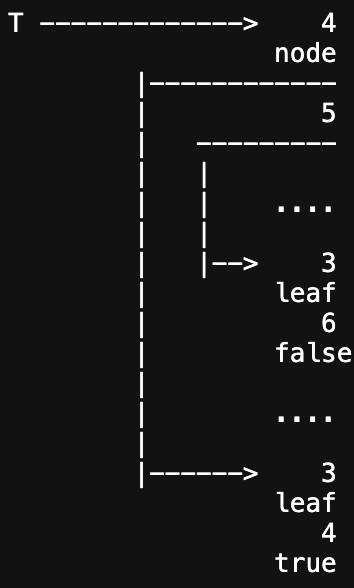
\includegraphics[width=0.25\textwidth]{img/t.png}
\end{center}
Per ogni tipo di dato boxed, il primo valore indica la dimensione della struttura dati.

Consideriamo ora una funzione che utilizza il pattern matching:
\begin{center}
    \texttt{f(\{\_, T1, 5, \{leaf, K, V\}\}) -> \{node, T1, 7, \{leaf, K, V\}\}}
\end{center}
Come viene compilato questo pattern?

Prendiamo come riferimento la seguente funzione:
\begin{center}
    \texttt{[| pattern, p |]}
\end{center}
dove \texttt{pattern} rappresenta il pattern della funzione,\\
\texttt{p} è il dato (equivalente a una word),\\
e \texttt{[| .,. |]} è una funzione eseguita a tempo di compilazione (che genera codice).

Esaminiamo i possibili casi di questa funzione:
\begin{itemize}
    \item \texttt{[| \_, p |] = }: non produce alcun codice.
    \item \texttt{[| X, p |] = word X = p;}, viene quindi assegnata una word per il dato \texttt{p}.
    
    X è una nuova variabile. È importante notare che in Erlang, se si utilizza una variabile X già dichiarata o assegnata in un pattern, si intende il \textbf{valore} della variabile stessa.
    \item \texttt{[| k, p |] = if(p != k) return -1;}, dove \texttt{k} è una costante di un tipo atomico.
    \item \begin{verbatim}
[| P1 = P2, p |] =
    [| P1, p[1] |]
    [| P2, p[2] |]
\end{verbatim}
    \item \begin{verbatim}
[| P1, ..., Pn, p |] = 

    if(is_unboxed(p)) return -1;
    if(p[0].length != n) return -1;
    [| P1, p[1] |] 
    ...
    [| Pn, p[n] |]
\end{verbatim}
\vspace{5pt}
\end{itemize}

Riprendendo la struttura T precedente 
\begin{center}
    \texttt{f(\{\_, T1, 5, \{leaf, K, V\}\}) -> \{node, T1, 7, \{leaf, K, V\}\}}
\end{center}
il codice compilato sarà:
\begin{tcolorbox}
\begin{verbatim}
if(is_unboxed(T)) return -1;
if(T[0].length != 4) return -1;
word T1 = T[2];
if(5 != T[3]) return -1;
if(is_unboxed(T[4])) return -1;
if(T[4][0].length != 3) return -1;
if(leaf != T[4][1]) return -1;
word K = T[4][2];
word V = T[4][3];
\end{verbatim}
\end{tcolorbox}

Il costo computazionale del pattern matching è \textbf{O(n)} sia in spazio che in tempo, dove n rappresenta la lunghezza del pattern.

Il costo computazionale dell'allocazione del risultato è \textbf{O(n)} sia in spazio che in tempo, dove n è la lunghezza dell'espressione utilizzata nell'output.

In pratica, questi costi sono \textbf{O(1)} a run-time poiché n \textbf{non} è un parametro dell'input a run-time.

Ogni variabile che ha catturato un tipo di dato boxed ha generato \textbf{sharing}, condividendo il dato attraverso il suo puntatore. Questo meccanismo non causa problemi se e solo se il linguaggio di programmazione non consente mutabilità dello Heap.\vspace{14pt}\\
Nei linguaggi che supportano nativamente pattern matching profondi (Erlang/OCaml/Haskell), durante la compilazione delle dichiarazioni di funzioni \textbf{non} si compilano i pattern uno alla volta come spiegato finora.

Un esempio può essere:
\begin{center}
    \texttt{f(\{ node, \{ node, T1, K1, T2 \}, K, \{leaf, \_, \_\} \}) when K1 < K -> ... ;}

    \texttt{f(\{ leaf, \_, 0, \_ \}) -> ... ;}

    \texttt{f(\{ node, \{ node, T1, K1, T2 \}, K, \{node, T3, T4\} \}) -> ... ;}
\end{center}
Vogliamo ora compilare questo codice in modo efficiente.

La semantica del linguaggio stabilisce che viene utilizzato il primo pattern in ordine che corrisponde all'input. Tuttavia, questo approccio non è ottimale dal punto di vista computazionale.

Si consideri l'invocazione di \texttt{f(\{node, \{node, .., 3, ..\}, 5, \{node, .., .., ..\} \})}

Dopo aver testato il primo pattern, se dimenticassimo tutto e passassimo a testare il secondo e poi il terzo, ripeteremmo operazioni già eseguite.

Non possiamo permutare i pattern per ottenere un albero di decisioni più efficiente, perché altrimenti non manterremmo l'ordine corretto di valutazione.

Per risolvere questo problema si utilizza un automa a stati finiti modificato, dove ogni stato dell'automa codifica l'informazione già acquisita sull'input.

Con questo approccio, la complessità diventa \textbf{sub-lineare} rispetto alla somma delle lunghezze dei pattern.

\subsection*{Ricorsione}
Il principio fondamentale è che a run-time viene mantenuto uno \textbf{Stack} di \textbf{Record di Attivazione} per ogni chiamata di funzione. Per convenzione, lo Stack cresce verso il basso.\\
Un RA (record di attivazione) contiene:
\begin{itemize}
    \item Variabili locali
    \item Parametri della funzione
    \item Valore dei registri salvati
    \item Indirizzo del valore di ritorno (dove memorizzare l'output)
    \item Indirizzo di ritorno
\end{itemize}

Il costo in spazio e in tempo di una chiamata di funzione è \textbf{O(1)}.

Ipotizziamo uno scenario in cui si stia eseguendo una funzione \texttt{f()} e viene invocata una funzione \texttt{g()}. Il record di attivazione di \texttt{f()} deve contenere \textbf{tutta (e sola)} l'informazione necessaria per \textbf{completare} l'esecuzione di \texttt{f()} dopo che \texttt{g()} sarà terminata.\\
In questo caso, non tutte le informazioni contenute nel record di attivazione di \texttt{f()} sono necessarie dopo la chiamata di \texttt{g()}.

Un esempio di questo caso può essere:

\begin{tcolorbox}
\begin{verbatim}
f(int x, int y, int p) {
    int z, w;
    ...
    g();
    p = y * z;
    return p + p;
}
\end{verbatim}
\end{tcolorbox}

Il record di attivazione di \texttt{f} contiene:
\begin{verbatim}
*w
z
p
y
*x
REGISTRI
RETURN VALUE
RETURN ADDRESS
\end{verbatim}
dove le variabili contrassegnate con * indicano variabili che non sono più necessarie dopo un certo punto dell'esecuzione, come si evince dal codice della funzione.

L'ottimizzazione consiste nel rimuovere le variabili non più necessarie dallo stack. Prima di invocare \texttt{g()}, lo stack pointer viene decrementato per liberare lo spazio occupato da \texttt{w}, ormai non più necessaria.

Inoltre, mediante un'analisi statica, è possibile determinare che sia più conveniente posizionare \texttt{x} subito dopo \texttt{w} nel record di attivazione, in modo da rilasciare anche lo spazio occupato da \texttt{x}.

Prolog, ad esempio, implementa sistematicamente queste ottimizzazioni.\vspace{14pt}\\
Esaminiamo ora un caso limite di questo approccio, definito \textbf{Tail Calls} (chiamate di coda).

Definizione: una chiamata a \texttt{g()} all'interno di \texttt{f()} è considerata di coda se e solo se:
\begin{itemize}
    \item L'unica istruzione eseguita \textbf{dopo} la chiamata a \texttt{g()} è un'istruzione di return.
    \item Il valore restituito dalla funzione \texttt{f()} è \textbf{esattamente} il valore restituito dalla funzione \texttt{g()}.
\end{itemize}

Quando una chiamata è identificata come chiamata di coda, viene compilata come:
\begin{tcolorbox}
\begin{verbatim}
pop(registri, variabili locali);
push(parametri attuali della g);
JUMP(codice della g);
\end{verbatim}
\end{tcolorbox}
La prima parte del record di attivazione della funzione \texttt{g()} coincide con la prima parte del record di attivazione della funzione \texttt{f()}.

Una chiamata di coda, quando è implementata la \textbf{Tail Call Optimization}, ha un costo di \textbf{O(1)} in tempo e \textbf{"O(0)"} in spazio (poiché viene riutilizzato il record di attivazione).

Un'ulteriore definizione, più diffusa ma meno precisa, è la seguente: una funzione \texttt{f()} si definisce \textbf{Tail Ricorsiva} se e solo se tutte le sue chiamate ricorsive sono chiamate di coda.

\subsection*{Eccezioni}
Fino ad ora, uno \textbf{stack frame} è sempre stato equivalente ad un \textbf{record di attivazione}.\\
Con l'introduzione delle eccezioni, uno stack frame può corrispondere a un record di attivazione oppure ad un \textbf{record try catch}.

All'interno di un record try catch troviamo un \textbf{puntatore al codice catch} ed un \textbf{tag "record try catch"}.

Un record di attivazione, invece, contiene i campi standard discussi in precedenza e un \textbf{tag "record di attivazione"}.

\pagebreak

Cosa accade quando viene eseguita una throw(E)? Ecco una possibile implementazione in pseudo-codice:
\begin{tcolorbox}
\begin{verbatim}
throw(E) {
 finished = false;
 while(!finished){
    while(Stack[0].TAG != "record try-catch") Stack.pop();

    addr = Stack[0].indirizzo_codice_catch
    Stack.pop();
    case CALL addr(E) of
      {catched, V} -> finished = true; V
      not_catched -> nothing
 }
}
\end{verbatim}
\end{tcolorbox}
\vspace{8pt}
Nota: a basso livello, il codice dopo il catch analizza le varie eccezioni e:
\begin{itemize}
    \item Se è in grado di gestirla, restituisce \texttt{\{catched, E\}} per un qualche valore \texttt{E}, oppure esegue un'altra \texttt{throw()} (in tal caso andrebbe modificato lo pseudo-codice precedente).
    \item Se non è in grado di gestirla, restituisce \texttt{not\_catched}.
\end{itemize}
\vspace{10pt}
Osserviamo ora un esempio di codice Erlang:
\begin{tcolorbox}
\begin{verbatim}
cc(Bal) ->
 try
  receive
    print -> io:format("Il balance è ~p ~n", [Bal]), cc(Bal) ;
                                                     ^^^^^^^
                                                chiamata non di coda
    {put, N} -> cc(Bal+N) ;
    {tax, N} -> cc(Bal / N) ;
    {get, PID} -> PID ! Bal, cc(Bal) ;
    exit -> ok
  catch
   error:_ -> cc(Bal)               % gestisco la divisione per zero
              ^^^^^^
          chiamata di coda
  end
 end.
\end{verbatim}
\end{tcolorbox}
\vspace{8pt}
In questo esempio, l'obiettivo è gestire la divisione per zero che può verificarsi durante il pattern matching sulla clausola \texttt{tax}.

È necessario quindi aggiornare la definizione di chiamata di funzione di coda.\\
\\Una chiamata di funzione è considerata di coda quando:
\begin{itemize}
    \item L'unica istruzione eseguita \textbf{dopo} la chiamata a \texttt{g()} è un'istruzione di return.
    \item Il valore restituito dalla funzione \texttt{f()} è \textbf{esattamente} il valore restituito dalla funzione \texttt{g()}.
    \item Non è contenuta all'interno della parte valutativa di un blocco \texttt{try ... catch} (ovvero non è protetta).
\end{itemize}
\vspace{8pt}
Vediamo ora come aggiornare il codice in una versione tail-ricorsiva:
\begin{tcolorbox}
\begin{verbatim}
cc(Bal) ->
  case
   try
    receive
      print -> io:format("Il balance è ~p ~n", [Bal]), {recur, Bal} ;
      {put, N} -> {recur, Bal+N} ;
      {tax, N} -> {recur, Bal / N} ;
      {get, PID} -> PID ! Bal, {recur, Bal} ;
      exit -> {result, ok}
   catch
    error:_ -> {recur, Bal}         % gestisco la divisione per zero
   end
  of
   {result, R} -> R ;
   {recur, Bal} -> cc(Bal) ;        % tail ricorsiva!
 end.
\end{verbatim}
\end{tcolorbox}
\vspace{8pt}
In questo modo attiviamo l'ottimizzazione della tail-ricorsione.

Una possibile riscrittura della struttura del codice (zucchero sintattico) può essere:
\begin{tcolorbox}
\begin{verbatim}
try
  E                                 % codice protetto
of
  p1 -> c1 ;                        % codice NON protetto
  ...                               % che fa match con il risultato di E
  pn -> cn ;
catch
 .... ->  ....                      % codice non protetto
\end{verbatim}
\end{tcolorbox}

\pagebreak

Applicando questa struttura al codice precedente otteniamo:
\begin{tcolorbox}
\begin{verbatim}
cc(Bal) ->
 try
  receive
    print -> io:format("Il balance è ~p ~n", [Bal]), {recur, Bal} ;
    {put, N} -> {recur, Bal+N} ;
    {tax, N} -> {recur, Bal / N} ;
    {get, PID} -> PID ! Bal, {recur, Bal} ;
    exit -> {result, ok}
 of
  {result, R} -> R ;
  {recur, Bal} -> cc(Bal) ;         % tail ricorsiva!
 catch
  error:_ -> {recur, Bal}           % gestisco la divisione per zero
 end.
\end{verbatim}
\end{tcolorbox}
\vspace{14pt}
È importante notare che Erlang non è un linguaggio completamente puro.

Un \textbf{linguaggio di programmazione puro} è un linguaggio che aderisce rigorosamente a un paradigma di programmazione specifico senza deviazioni. Generalmente, il termine si riferisce ai linguaggi funzionali puri, che rispettano il modello della programmazione funzionale senza effetti collaterali. Le caratteristiche principali sono:
\begin{itemize}
    \item \textbf{Assenza di effetti collaterali}: le funzioni non modificano lo stato globale o variabili esterne. Il risultato di una funzione dipende esclusivamente dai suoi input.
    \item \textbf{Trasparenza referenziale}: una funzione restituisce sempre lo stesso output per gli stessi input, indipendentemente dal contesto di esecuzione.
    \item \textbf{Immutabilità dei dati}: le variabili non possono essere modificate dopo la loro assegnazione. Si utilizzano strutture dati immutabili.
    \item \textbf{Lazy evaluation}: le espressioni vengono valutate solo quando necessario, migliorando efficienza e modularità.
    \item \textbf{Funzioni di prima classe e di ordine superiore}: le funzioni possono essere passate come parametri e restituite come valori.
    \item \textbf{Composizione funzionale}: le funzioni possono essere combinate per creare nuove funzioni senza necessità di strutture di controllo imperative.
\end{itemize}
Un esempio paradigmatico di linguaggio puro è \textit{Haskell}.\vspace{14pt}\\
Erlang permette l'accesso al file system tramite specifici costrutti. Naturalmente, una volta aperto un file, sarà necessario chiuderlo al termine del suo utilizzo. Un'eccezione potrebbe interrompere un'esecuzione corretta e causare problemi.

\pagebreak

Un possibile codice per la gestione di un file può essere:
\begin{tcolorbox}
\begin{verbatim}
FD = open(...);
try
 ....                               % throw(exc2)
 close(FD)
catch
 exc1 -> close(FD), 4
 _:_ = R -> close(FD), throw(R)    % CODICE NON DEL TUTTO CORRETTO
end
\end{verbatim}
\end{tcolorbox}
\vspace{8pt}
Per risolvere questa problematica è necessario un nuovo costrutto.

Come in altri linguaggi di programmazione, esiste il costrutto \texttt{finally} (in Erlang denominato \texttt{after}).

Riprendendo la struttura precedente e aggiungendo il nuovo costrutto \texttt{after}:
\begin{tcolorbox}
\begin{verbatim}
try
  E
of
  F
catch
  G
after C
end
\end{verbatim}
\end{tcolorbox}
\vspace{8pt}
Una possibile implementazione in pseudo-codice può essere:
\begin{tcolorbox}
\begin{verbatim}
case
 try
  {return, try E of F catch G}      % tutte le chiamate sono protette
 catch                              % e quindi non di coda
  Exc -> {exception, Exc}
 end
of
 {return, V} -> C, V ;
 {exception, Exc} -> C, throw(Exc)
end.
\end{verbatim}
\end{tcolorbox}
\vspace{8pt}
È importante sottolineare che quando si utilizza il costrutto \texttt{after}, si perde completamente l'ottimizzazione delle chiamate di coda.

\pagebreak

In Erlang esistono tre tipologie di eccezioni:
\begin{itemize}
    \item \texttt{throw()}: corrisponde al passaggio al \textit{control operator}. Le eccezioni lanciate con \texttt{throw} non sono concepite come errori, ma semplicemente come meccanismo per il passaggio di controllo.
    \item \texttt{exit()}: interrompe l'esecuzione dell'attore. Viene utilizzata per implementare la filosofia di Erlang \textit{Let it fail}. Queste eccezioni non dovrebbero essere catturate con \texttt{catch}.
    \item \textit{Errori non risolvibili}: in questi casi non ha senso far ripartire l'attore, a causa di codice non implementato correttamente. In altri linguaggi equivalgono ad errori di compilazione. In queste situazioni viene fornito lo \textit{stack trace} dell'errore.
\end{itemize}
\vspace{8pt}
Esistono inoltre altri tre costrutti considerati deprecati o di utilizzo limitato:
\begin{itemize}
    \item \texttt{(catch throw(pippo))}: deprecato, utilizzato prima dell'introduzione del nuovo costrutto try catch descritto in precedenza. Non consente di distinguere il tipo di eccezione.
    \item \texttt{if}: forma semplificata di pattern matching, dove è possibile utilizzare esclusivamente \textit{guardie}.
    \item \texttt{= (uguale)}: esegue un pattern matching tra la parte sinistra e quella destra. Quando i due pattern corrispondono si parla di \textit{pattern irrefutabile}. Se viene utilizzato un pattern irrefutabile ma il match fallisce, viene generato un errore.
\end{itemize}

\pagebreak

\subsection*{Algebraic Effects}
Gli Algebraic Effects si basano su un concetto fondamentale: l'istruzione \texttt{throw(E)} trasferisce il controllo a distanza alla clausola \texttt{catch} che gestisce l'effetto \texttt{E}. Il codice remoto può successivamente restituire il controllo alla \texttt{throw} fornendo un valore \texttt{V} che diventa il risultato dell'istruzione \texttt{throw} stessa.

Un esempio in pseudo codice Erlang potrebbe essere:
\begin{tcolorbox}
\begin{verbatim}
2 * try 3 + (5 + throw 7)
    catch
        0 -> 22                     % come un'eccezione normale
        N -> resume N+1             % resume nuova keyword
    end
\end{verbatim}
\end{tcolorbox}
Nel caso dell'utilizzo di resume, il risultato sarebbe \texttt{32}.

Come viene implementato questo meccanismo di "ritorno"?\\
Nelle eccezioni tradizionali, la \texttt{throw} esegue un ciclo \texttt{while} sullo stack e per ogni record di attivazione/record try catch che non gestisce l'eccezione effettua \texttt{Stack.pop()}.

Negli algebraic effects (nell'implementazione più semplice) la \texttt{throw}, invece di eseguire un semplice \texttt{Stack.pop()}, effettua:
\begin{tcolorbox}
\begin{verbatim}
RA = Stack.pop();
Detached.push(RA);
\end{verbatim}
\end{tcolorbox}
dove Detached rappresenta un secondo stack, ordinato in senso inverso, nel quale vengono temporaneamente memorizzati i frame di stack distaccati.

L'istruzione \texttt{resume} esegue la seguente operazione:
\begin{tcolorbox}
\begin{verbatim}
while(!Detach.is_empty()) {
    RA = Detach.pop();
    Stack.push(RA);
}
\end{verbatim}
\end{tcolorbox}
assegnando il risultato della \texttt{resume} come valore di ritorno della \texttt{throw}.

Se invece nel ramo \texttt{catch} non viene utilizzata l'istruzione \texttt{resume}:
\begin{tcolorbox}
\begin{verbatim}
while(!Detach.is_empty())
    Detach.pop()
\end{verbatim}
\end{tcolorbox}
\vspace{8pt}
In un linguaggio con supporto per gli effetti algebrici viene introdotto un nuovo tipo di dato astratto denominato \textbf{fibra} (\textbf{fiber}) che rappresenta un frammento di stack distaccato. Questo è un tipo di dato di prima classe sul quale è possibile invocare l'operazione \texttt{resume()} per reinstallarlo in cima allo stack corrente. Il ramo \texttt{catch} cattura questa fibra.

Esaminiamo ora un esempio di implementazione di uno scheduler, in pseudo codice Erlang:
\begin{tcolorbox}
\begin{verbatim}
yield() -> throw(yield).            % yield è un effetto
fork(G) -> throw(fork).             % fork è un effetto

code_to_fiber(F) ->
 try
  throw(stop),F
 catch
  stop, K -> K
 end.

% Main è il primo thead da eseguire
% Queue la coda dei thread sospesi
scheduler(Main, Queue) ->
 try
  resume(Main, ok)
 catch
  yield, K ->                      % K è la fibra, i pattern sono sempre
   case Queue of                   % pattern_eccezione + pattern K
    [] -> scheduler(K, [])
    [F|L] -> scheduler(F, append(L,[K]))
   end ;
  fork(G), K ->
    scheduler(K, append(Queue,[code_to_fiber(G)]))
 end.

scheduler(Main) ->
 scheduler(code_to_fiber(Main),[]).
\end{verbatim}
\end{tcolorbox}
\vspace{8pt}
Gli effetti algebrici consentono quindi di gestire in maniera non locale gli errori come se fossero gestiti localmente, di implementare scheduler a livello utente (user-space), e altri meccanismi avanzati.

Un'implementazione efficiente degli effetti algebrici trasforma lo stack in uno stack di fibre, dove ogni fibra è a sua volta uno stack.\\
In questo modo, le operazioni di distacco e riattacco di una fibra hanno un costo computazionale di \textbf{O(1)}, sebbene ciò comporti che lo stack non sia più allocato in modo contiguo in memoria.

\pagebreak

\subsection*{Gestione della memoria}
In un linguaggio di programmazione sequenziale emergono diverse problematiche nella gestione della memoria:
\begin{itemize}
    \item Formazione del \textbf{Garbage} (memoria non deallocata non più utile, la cui utilità è \textit{indecidibile} a livello teorico).
    \item Puntatori a memoria non allocata (dangling pointers).
    \item Riutilizzo improprio di memoria deallocata. Si suddivide in due casi:
    \begin{itemize}
        \item Accesso alla memoria già deallocata.
        \item Ri-deallocazione della memoria già deallocata (double free).
    \end{itemize}
    \item Frammentazione della memoria.
    \item Memoria non allocata.
\end{itemize}

Nell'ambito concorrente/parallelo, a queste problematiche se ne aggiungono altre. Un esempio significativo è la \textbf{Race Condition}, situazione in cui il risultato della computazione dipende dall'ordine di esecuzione dei programmi. Questo può verificarsi in diversi scenari, come quando un thread opera in scrittura mentre altri thread leggono contemporaneamente lo stesso dato.\\
Il programmatore deve gestire attentamente questi casi, implementando meccanismi di sincronizzazione come i vari sistemi di locking.

Consideriamo ora un esempio di funzione in \textit{C}:
\begin{center}
    \texttt{T f(..., T x);}
\end{center}
dove \texttt{T} rappresenta un tipo di dato generico. In assenza di informazioni sul tipo di dato, possono presentarsi diverse problematiche inerenti alla memoria:
\begin{enumerate}
    \item Il dato \texttt{T} in output è interamente allocato ad ogni chiamata. 
    
    Non esistono puntatori che collegano input ad output (o viceversa), né puntatori dal dato a variabili globali (dichiarate a top-level, accessibili senza averle prese in input e disponibili anche dopo l'esecuzione della funzione) o statiche (simili alle variabili globali, ma con visibilità limitata all'interno della funzione).
    
    Solo il chiamante della funzione ha accesso al dato. Sarà quindi responsabilità del chiamante determinare se il dato è ancora utile.
    \item L'input è condiviso con l'output.
    
    Esistono puntatori dall'output all'input. In questo caso, l'input non può essere considerato garbage finché l'output non lo diventa.
    \item L'output è condiviso con l'input (caso opposto al precedente).
    
    Esistono puntatori dall'input all'output. In questo caso, l'output non può essere considerato garbage finché l'input non lo diventa.
    \item Combinazione del punto \textit{2} e del punto \textit{3}. Input e output devono diventare garbage contemporaneamente.
    \item La funzione mantiene un puntatore all'output (o a parte di esso). 
    
    Esempi di questo caso sono gli oggetti \textit{Singleton} e il pattern \textit{Memoization} (dove i risultati per diversi input vengono memorizzati all'interno di una hash table).

    L'output non può essere considerato garbage finché non lo sono tutti gli output precedenti e quell'input non verrà più richiesto.
\end{enumerate}
Tutti questi casi possono verificarsi nella funzione descritta precedentemente.\vspace{14pt}\\
Esistono diverse tecniche per la gestione della memoria:
\begin{itemize}
    \item Nessuna gestione automatica della memoria (come in C).
    \item Garbage collection automatica. 
    
    Il run-time del linguaggio cerca di approssimare l'utilità di un dato e dealloca i dati che considera garbage.
    
    Viene implementata un'\textit{euristica} di garbage detection, la cui efficacia varia in base all'algoritmo scelto. In alcuni casi, il programmatore può assistere l'euristica per ottimizzare il riconoscimento del garbage.

    Questa tecnica si divide in due principali categorie:
    \begin{itemize}
        \item Reference Counting
        \item Mark \& Sweep
    \end{itemize}
    \item Gestione esplicita da parte del programmatore (come in Rust, C++).
    
    Non è presente alcuna euristica di garbage detection, ma è il programmatore che esplicitamente descrive al compilatore gli invarianti di accesso ai dati.\\
    Il compilatore inserisce quindi il codice necessario per gestire allocazione/deallocazione in base alle specifiche fornite dal programmatore.\vspace{8pt}
\end{itemize}

\textbf{Reference Counting}\\
L'euristica del reference counting si basa sul principio che: \textit{se un dato boxed ha 0 puntatori entranti, allora il dato è garbage.}

Per applicare questa euristica è necessario tenere traccia, per ogni dato boxed, del numero di puntatori entranti.

A tal fine, nella prima cella del dato boxed, insieme al tag e al numero di celle (dimensione del dato), viene memorizzato anche un \textbf{Reference Counter} (\textbf{RC}), ovvero un numero intero che conteggia i puntatori entranti.\\
Questo valore deve essere maggiore di 0, altrimenti il dato viene considerato garbage e deallocato.

L'euristica utilizzata in questo caso, pur essendo efficace, non è ottimale in tutte le situazioni.

È importante introdurre il concetto di \textbf{radice}. Le radici sono celle di memoria sempre accessibili al programma, come lo stack e i registri.

Un problema significativo del reference counting si verifica quando il contatore non può arrivare a 0, impedendo la deallocazione, come nel caso di strutture dati con riferimenti ciclici (ad esempio, una lista doppiamente linkata). In questi casi si crea garbage ogni volta che si perde il puntatore alla prima cella della lista.

Per risolvere il problema delle strutture dati cicliche, viene introdotto il concetto di \textbf{weak pointer}, distinguendolo dai normali puntatori ora denominati \textbf{strong pointer}.

Nel caso di liste doppiamente linkate, i puntatori strong vengono utilizzati per riferirsi alla cella successiva nella lista, mentre i puntatori weak vengono impiegati per riferirsi all'elemento precedente.

Grazie a questa distinzione, nel reference counter vengono conteggiati solo i puntatori strong, consentendo una gestione più efficace della garbage detection.

Questo metodo, tuttavia, non risolve completamente le problematiche menzionate in precedenza. L'utilizzo dei puntatori weak richiede una gestione attenta da parte del programmatore. 

Inoltre, è necessario prestare particolare attenzione ai puntatori weak che potrebbero riferirsi a celle già deallocate. In questo caso, sono necessarie strutture dati aggiuntive per verificare se il puntatore weak si riferisce ancora a un dato allocato.

\vspace{14pt}
Analizziamo ora le operazioni di allocazione e gestione dei dati:
\begin{itemize}
    \item La memoria è frammentata: sono necessari algoritmi efficaci per la gestione del pool di aree di memoria libera (come Best Fit, First Fit, ecc.). Questo processo ha un costo significativo in termini di spazio/tempo. Una possibile implementazione può essere:
    
\begin{tcolorbox}
\begin{verbatim}
p = alloc(size + 1);        // + 1 per la presenza della cella RC
(*p)[0] = 1;
\end{verbatim}
\end{tcolorbox}

    Quando viene allocata una cella, il RC è inizializzato a 1, indicando che esiste un solo riferimento entrante.
    \item Copia di un puntatore. Una possibile implementazione può essere:

\begin{tcolorbox}
\begin{verbatim}
if(q != null) {
    (*q)[0]--;

    if((*q)[0] == 0) {
        dealloc(q);
    }
}

q = p;
(*p)[0]++;
\end{verbatim}
\end{tcolorbox}

    È necessario aggiornare il valore RC di \texttt{q} quando un puntatore viene copiato in quella variabile. Questo può causare una deallocazione a cascata.
    
    Una possibile implementazione di \texttt{dealloc()} può essere, in pseudo codice:
\begin{tcolorbox}
\begin{verbatim}
dealloc(q) {
    for i = 1 to (*q)[0].size do {
        if(boxed (*q)[i]) {
            (*q)[i]--;

            if((*q)[i] == 0) {
                dealloc((*q)[i]);
            }
        }
    }
    free(q);
}
\end{verbatim}
\end{tcolorbox}

    Il costo computazionale della copia di un puntatore risulta proporzionale alla lunghezza della catena di deallocazioni, potenzialmente pari al numero totale di operazioni eseguite dal programma fino a quel momento (definito come \textbf{unbounded}).

    Il costo in tempo è quindi \textbf{O(n)}, dove \texttt{n} rappresenta il numero di passi del programma.
\end{itemize}

\vspace{14pt}
\textbf{Mark \& Sweep}\\
L'euristica del mark \& sweep, nella sua versione base, afferma che: \textit{un dato non raggiungibile dalle radici viene considerato garbage}.

La fase di \textbf{Mark} parte dalle radici e \textit{marka} con dei bit tutto quello che è raggiungibile. Tutto il resto viene considerato garbage.

La fase di \textbf{Sweep} invece effettua una sorta di deframmentazione. Tutte le celle markate vengono spostate e deframmentate, mentre le celle non spostate vengono deallocate.

Continuare con lezione 11 marzo.

\end{document}